\documentclass[../NormediProgetto.tex]{subfiles}


\begin{document}

% NORME DI PROGETTO - PROCESSI DI SUPPORTO

\chapter{Processi di supporto}

% NORME DI PROGETTO - PROCESSI DI SUPPORTO - GESTIONE DELLA CONFIGURAZIONE

\section{Documentazione}

\subsection{Scopo} 

Lo scopo del processo di documentazione è descrivere l'insieme di regole adottate dal gruppo per la redazione della documentazione di progetto. Il gruppo si prefigge di definire in questo capitolo norme atte alla stesura di una documentazione il più possibile formale, corretta, coerente e coesa.

\subsection{Produzione Documentale}
Durante il corso del progetto è richiesta la stesura dei seguenti documenti:
\begin{longtable}{| p{4cm} |p{5cm} | p{4cm} |}
	\caption {Tabella produzione documentale} \label{tab:title} \\
	\hline
	\textbf{Processo} & \textbf{Attività} & \textbf{Documento} \\
	\hline
	\endhead
	
	\newline Fornitura &
	\newline Analisi dei capitolati &
	\newline Studio di fattibilità \newline 
	\\[1em]
	
	\hline
	
	\newline Fornitura &
	\newline Definizione del ciclo di sviluppo &
	\newline Piano di Progetto \newline 
	\\[1em]
	
	\hline
	
	\newline Fornitura &
	\newline Pianificazione della qualità &
	\newline Piano di Qualifica \newline 
	\\[1em]
	
	\hline
	
	\newline Sviluppo &
	\newline Analisi dei requisiti &
	\newline Analisi dei requisiti \newline 
	\\[1em]
	
	\hline
	
	\newline Sviluppo &
	\newline Progettazione  &
	\newline Product Baseline  
	\newline Prima bozza manuali \newline
	\\[1em]
	
	\hline
	
	\newline Sviluppo &
	\newline Codifica &
	\newline Manuali\newline 
	\\[1em]
	
	\hline
	
	\newline Gestione di progetto &
	\newline Gestione degli incontri &
	\newline Verbali \newline 
	\\[1em]
	
	\hline
\end{longtable}

\noindent Durante l'intero svolgimento del progetto verrà redatto e incrementato un Glossario.

% STRUTTURA DEI DOCUMENTI

\subsection{Struttura dei documenti}

\subsubsection{Template}

Il gruppo utilizza un template \LaTeX{} appositamente codificato per uniformare l'aspetto dei documenti e velocizzare il processo di documentazione. Il template include frontespizio, registro delle modifiche, indice, piè di pagina e intestazione, elementi del documento approfonditi di seguito. 

\subsubsection{Frontespizio}

Il frontespizio di ogni documento è strutturato nel seguente modo:

\begin{itemize}
	\item \textbf{Logo del gruppo:} il logo identificativo del gruppo;
	\item \textbf{Nome del documento:} indica il nome del documento (ex: Norme di progetto);
	\item \textbf{Informazioni sul documento:} tabella riassuntiva indicante le seguenti informazioni di spicco sul documento:
	\begin{itemize}
		\item \textbf{Versione:} indica un numero che identifica la versione corrente del documento. La struttura del numero di versionamento è approfondita di seguito in questa sezione;
		\item \textbf{Data di approvazione:} indica l'ultima data in cui il documento è stato approvato;
		\item \textbf{Responsabile:} indica il Responsabile che ha approvato il documento;
		\item \textbf{Redattori:} indica il sottoinsieme dei membri del gruppo che ha partecipato alla redazione del documento;
		\item \textbf{Verificatori:} indica il sottoinsieme dei membri del gruppo che ha partecipato alla verifica del documento;
		\item \textbf{Distribuzione:} indica a chi è destinato il documento;
		\item \textbf{Uso:} indica se l'uso del documento è interno o esterno al gruppo;          
		\item \textbf{Recapito:} la mail di recapito del gruppo
	\end{itemize}
	
\end{itemize}

\subsubsection{Nomenclatura di versionamento dei documenti}
Ogni documento è accompagnato da un numero di versionamento, indicato nella tabella \textit{Informazioni sul documento}, dove ogni versione corrisponde ad una riga nel registro delle modifiche, che è espresso nel modo seguente:

\[\textbf{v $\biggl\{$A$\biggr\}$.$\biggl\{$B$\biggr\}$.$\biggl\{$C$\biggr\}$}\]

Dove:

\begin{itemize}
	\item{\textbf{A:}} è l'indice principale. Viene incrementato dal \textit{Responsabile di Progetto} all’approvazione del documento e 
	corrisponde al numero di revisione.
	\item{\textbf{B:}} è l'indice di verifica. Viene incrementato dal \glossario{\textit{Verificatore}}{verificatore} ad ogni verifica. Quando viene incrementato A, riparte da 0.
	\item{\textbf{C:}} è l'indice di modifica. Viene incrementato dal redattore del documento ad ogni modifica. Quando viene incrementato B, riparte da 0.
\end{itemize}

\subsubsection{Registro delle modifiche}

Dopo il frontespizio segue il registro delle modifiche, che cataloga le modifiche apportate al documento durante il suo sviluppo indicando per ognuna:

\begin{itemize}
	\item Versione del documento dopo la modifica;
	\item Data della modifica;
	\item Nome e cognome dell'autore della modifica;
	%\item Ruolo dell'autore della modifica;
	\item Breve descrizione della modifica.
\end{itemize}

\subsubsection{Indice}

Ogni documento possiede un indice che ne agevola la consultazione e permette una visione generale degli argomenti trattati nello stesso. L'indice è strutturato gerarchicamente ed è collocato dopo il registro delle modifiche.

\subsubsection{Intestazione}

Fatta eccezione per il frontespizio, tutte le pagine del documento contengono un’intestazione. Questa è costituita da: 

\begin{itemize}
	\item \textbf{Logo del gruppo:} il logo identificativo del gruppo Graphite, collocato a sinistra;
	\item \textbf{Titolo del capitolo:} indicazione del titolo del capitolo corrente, collocata a destra.
\end{itemize}

\subsubsection{Piè di pagina}

Fatta eccezione per il frontespizio, tutte le pagine del documento contengono un piè di pagina. Questo è costituito da: 

\begin{itemize}
	\item \textbf{Nome documento e versione:} indica il nome del documento e la sua versione attuale, collocate a sinistra;
	\item \textbf{Numero di pagina:} numerazione progressiva delle pagine, collocato a destra.
\end{itemize}

\subsubsection{Note a piè di pagina}

In caso di presenza in una pagina interna di note da esplicare, esse vanno indicate nella pagina corrente, in basso a sinistra. Ogni nota deve riportare un numero, corrispondente alla relativa parola o frase che la riferisce, e una descrizione.

\subsubsection{Contenuto principale}

Il contenuto principale del documento è organizzato secondo la seguente struttura gerarchica:

\begin{enumerate}
	\item Capitolo;
	\item Sezione;
	\item Sottosezione;
	\item Sottosottosezione.
\end{enumerate}

% NORME TIPOGRAFICHE

\subsection{Norme tipografiche}

\subsubsection{Stile del testo}

\begin{itemize}
	
	\item \textbf{Glossario:} ogni parola contenuta nel glossario deve essere marcata, solo alla sua prima occorrenza in ogni documento, in corsivo e con una G maiuscola a pedice. Tale formattazione viene assicurata dalla macro \textit{\textbackslash glossario\{termine\}\{riferimento al glossario\}} che stampa il termine con la giusta formattazione (\textit{termine}\ped{G}) e controlla che il suo riferimento sia presente nel glossario, restituendo un errore di compilazione in caso contrario, il termine di riferimento è la parola in minuscola senza accenti;  
	
	\item \textbf{Grassetto:} il grassetto viene applicato ai titoli e agli elementi di un elenco puntato seguiti da una descrizione. Esso può inoltre essere usato per mettere in particolare risalto termini significativi; 
	
	\item \textbf{Corsivo:} il corsivo viene utilizzato per:
	\begin{itemize}
		\item citazioni;
		\item termini di glossario;
		\item attività del progetto;
		\item ruoli del progetto;
		\item riferimenti ad altri documenti.
	\end{itemize}
	
	Esso può inoltre essere usato per mettere in particolare risalto termini particolari solitamente poco usati o conosciuti;
	
	\item{\textbf{Maiuscolo:}} il maiuscolo viene usato solo per gli acronimi.
	
\end{itemize}

\subsubsection{Elenchi puntati}

Gli elenchi puntati servono ad esprimere in modo sintetico un concetto, evitando frasi lunghe e dispersive. Ogni voce di un elenco puntato termina con un punto e virgola, ad eccezione dell'ultima, che termina invece con un punto.

\subsubsection{Formati}

\begin{itemize}
	
	\item{\textbf{Date:}}  \[\textbf{AAAA-MM-GG}\]
	\begin{itemize}
		\item{\textbf{AAAA:}} rappresenta l'anno in cifre per intero;
		\item{\textbf{MM:}} rappresenta il mese in cifre;
		\item{\textbf{GG:}} rappresenta il giorno del mese in cifre.
		
	\end{itemize}
	
	\item{\textbf{Orari:}} \[\textbf{HH:MM}\]
	\begin{itemize}
		\item{\textbf{HH:}} rappresenta l'ora;
		\item{\textbf{MM:}} rappresenta i minuti.
	\end{itemize}
	
	\item{\textbf{Nomi ricorrenti:}}
	\begin{itemize}
		\item{\textbf{Ruoli di progetto:}} ogni nome di ruolo di progetto viene scritto in corsivo e con l’iniziale maiuscola;
		\item{\textbf{Nomi dei documenti:}} ogni nome di documento viene scritto in corsivo e con l’iniziale di ogni parola che non sia un articolo maiuscola;
		\item{\textbf{Nomi propri:}} ogni nome proprio di persona deve essere scritto nella forma \textit{Nome Cognome}.
	\end{itemize}
	
	\item{\textbf{Link:}} i link esterni devono essere scritti attraverso il comando \LaTeX{} \textit{url} e sono distinti dal colore blu. I link interni, per esempio quelli dell'indice, non vengono evidenziati.
\end{itemize}

\subsubsection{Sigle}

È previsto l’utilizzo delle seguenti sigle: 

\begin{itemize}
	\item{\textbf{AR:}} \textit{Analisi dei Requisiti};
	\item{\textbf{PP:}} \textit{Piano di Progetto};
	\item{\textbf{NP:}} \textit{Norme di Progetto};
	\item{\textbf{SF:}} \textit{Studio di Fattibilità};
	\item{\textbf{PQ:}} \textit{Piano di Qualifica};
	\item{\textbf{TB:}} \glossario{Technology Baseline}{Technology Baseline};
	\item{\textbf{MU:}} \glossario{Manuale utente}{manuale utente};
	\item{\textbf{MS:}} \glossario{Manuale sviluppatore}{manuale sviluppatore};
	\item{\textbf{PB:}} \glossario{Product Baseline}{Product Baseline};
	\item{\textbf{PoC:}} \textit{Proof of Concept};
	\item{\textbf{RR:}} Revisione dei requisiti;
	\item{\textbf{RP:}} Revisione di progettazione;
	\item{\textbf{RQ:}} Revisione di qualifica;
	\item{\textbf{RA:}} Revisione di accettazione;
	\item{\textbf{Re:}} \textit{Responsabile di Progetto};
	\item{\textbf{Am:}} \textit{Amministratore di Progetto};
	\item{\textbf{An:}} \textit{Analista};
	\item{\textbf{Pt:}} \textit{Progettista};
	\item{\textbf{Pr:}} \glossario{Programmatore}{programmatore};
	\item{\textbf{Ve:}} \textit{Verificatore}.
\end{itemize}

\subsection{Elementi grafici}

\subsubsection{Tabelle}

Ogni tabella è corredata da una didascalia in cui compare il suo numero identificativo (per agevolarne il tracciamento) ed una breve descrizione del suo contenuto.

\subsubsection{Immagini}

Ogni immagine deve essere centrata e separata dai paragrafi a lei precedenti e successivi. Le immagini sono corredate da una didascalia analoga a quella delle tabelle. Tutti i diagrammi vengono inseriti come immagini.

\subsection{Classificazione dei documenti}

\subsubsection{Documenti informali}

Tutte le versioni dei documenti che non siano state approvate dal \textit{Responsabile di Progetto} sono ritenute informali e, in quanto tali, sono considerate esclusivamente ad uso interno.

\subsubsection{Documenti formali}

Una versione di un documento viene considerata formale quando è stata approvata dal \textit{Responsabile di Progetto}. Solo i documenti formali possono essere distribuiti all’esterno del gruppo.

\subsubsection{Documenti interni}

Un documento viene considerato interno quando il suo utilizzo è destinato al solo gruppo Graphite.

\subsubsection{Documenti esterni}

Un documento viene considerato esterno quando il documento viene condiviso con i Committenti e con la Proponente.

\subsubsection{Verbali}

Per ogni incontro interno o esterno è prevista la redazione di un verbale, contenente le seguenti informazioni:
\begin{itemize}
	\item \textbf{Informazioni sull'incontro:}
	\begin{itemize}
		\item \textbf{Luogo}: indica il luogo in cui si svolge la riunione. In caso di videochiamate, questo campo può essere riempito con la voce \textit{"Videochiamata"} e/o con il punto di ritrovo in cui si è svolta (ex: Aula AC150, Torre Archimede (Videochiamata));
		\item \textbf{Data:} indica la data in cui si è svolto l'incontro;
		\item \textbf{Orari:} indica orari di inizio e di fine dell'incontro;
		\item \textbf{Partecipanti del gruppo:} indica i membri del gruppo partecipanti all'incontro;
		\item \textbf{Partecipanti esterni:} indica, se dovessero essercene, eventuali partecipanti esterni presenzianti all'incontro.
	\end{itemize}
	
	\item \textbf{Ragioni dell'incontro:} indica le ragioni che hanno spinto ad indire l'incontro in esame. In questa sezione viene inserito l'eventuale ordine del giorno;
	
	\item \textbf{Resoconto:} contiene annotazioni riguardo gli argomenti discussi e capisaldi dell'incontro;
	
	\item \textbf{Tracciamento delle decisioni:} indica eventuali decisioni prese durante l'incontro, tracciate mediante il seguente codice:
	
	\[V[Tipologia]-[Data incontro].[ID]\]
	
	Dove:
	
	\begin{itemize}
		\item \textbf{Tipologia:} indica se il verbale è interno oppure esterno;
		\item \textbf{Data incontro:} indica la data in cui si è svolto l'incontro in formato \textit{AAAA-MM-GG};
		\item \textbf{ID:} è un codice identificativo numerico incrementale.
	\end{itemize}
	
\end{itemize}

\noindent I verbali dovranno essere approvati dal \textit{Responsabile di Progetto} al termine di ogni incontro.

\subsection{Ciclo di vita del documento}

Ogni documento non formale completato deve essere sottoposto al \textit{Responsabile di Progetto}, che si occupa di incaricare i \textit{Verificatori} di controllarne la correttezza del contenuto e della forma. Se vengono individuati degli errori, i \textit{Verificatori} li riportano al \textit{Responsabile di Progetto}, che a sua volta incarica il redattore del documento di correggerli. Questo ciclo va ripetuto fino a che il documento non è considerato corretto. Successivamente esso viene sottoposto al Responsabile di Progetto, che può o meno approvarlo. Quando approvato, il documento è da considerarsi formale. In caso contrario il \textit{Responsabile di Progetto} deve comunicare le motivazioni per cui il documento non è stato approvato, specificando le modifiche da apportare.

\subsection{Nomenclatura dei documenti}

I documenti formali, fatta eccezione per i Verbali di riunione, adottano il seguente sistema di nomenclatura:

\[NomeDelDocumento vX.Y.Z\]

Dove:

\begin{itemize}
	\item \textbf{NomedelDocumento:} indica il nome del documento, senza spazi con lettera maiuscola per ogni parola che non sia un articolo o una preposizione;
	
	\item \textbf{vX.Y.Z:}  indica l'ultima versione del documento approvata dal \textit{Responsabile di Progetto}.
\end{itemize}

\subsection{Formato dei file}
I file legati alla documentazione vengono salvati in formato .tex durante il loro ciclo di vita. Quando un documento raggiunge lo stato di "Approvato" viene creato un file in formato PDF contenente la versione del documento approvata dal \textit{Responsabile}.

\section{Gestione della configurazione}

\subsection{Versionamento} 
Ogni componente versionabile del progetto, nonché la documentazione formale, è versionata mediante la tecnologia \glossario{Git}{Git}, nello specifico utilizzando il servizio gratuito GitHub.
Per la condivisione di materiale informale e/o non versionabile si predilige invece una cartella condivisa sullo spazio cloud offerto da \glossario{Google Drive}{Google Drive}.

\subsection{Controllo della configurazione}

Per identificare e tracciare le richieste di cambiamenti, analizzare e valutare le modifiche effettuate e approvare o meno quelle proposte, viene utilizzato il sistema di \glossario{issue}{issue} di Github. Le issue riportano nella loro descrizione la ragione della modifica effettuata, nonché la o le \glossario{commit}{commit} ad esse associate ed eventuali ulteriori issue correlate. 

\subsection{Stato della configurazione}

Successivamente ad ogni revisione, l'ultima commit effettuata viene marcata con un'etichetta di versione (essa costituirà la nuova \glossario{baseline}{baseline} di riferimento). L'esito delle revisioni vengono riportate in appendice al PQ con le relative correzioni da apportare ai prodotti oggetto della revisione.

\subsection{Rilasci e consegne}

I rilasci e le consegne dei prodotti software e della documentazione correlata sono sottoposti a verifica e validazione. Prima di ogni revisione viene consegnato al \textit{Committente}, secondo tempistiche stabilite dal PP e mezzi concordati, un archivio contenente tutta la documentazione richiesta in formato \glossario{PDF}{PDF}. La consegna è accompagnata da una Lettera di
Presentazione, anch'essa inclusa nell'archivio.

% NORME DI PROGETTO - PROCESSI DI SUPPORTO - GESTIONE DELLA QUALITà

\section{Gestione della qualità}

\subsection{Scopo}
Il processo di gestione della qualità è finalizzato al conseguimento degli obiettivi di qualità definiti dal gruppo per garantire uno sviluppo efficace ed efficiente del prodotto richiesto.

% STANDARD QUALITATIVI DI RIFERIMENTO

\subsection{Definizione degli standard \\ qualitativi di riferimento}

Vengono di seguito sinteticamente esposti gli standard di qualità a cui il gruppo intende aderire e le motivazioni di tale scelta.   

\subsubsection{Qualità di processo - ISO/IEC 15504}

\glossario{ISO/IEC 15504}{ISO/IEC 15504}, anche noto come \glossario{SPICE}{SPICE}, è lo standard scelto per la definizione degli obiettivi di processo. Si rimanda all'appendice §A.1 del PQ per un'approfondita descrizione di tale standard.
La scelta di SPICE è motivata dal fatto che esso fornisce gli strumenti utili a valutare la qualità di processo, parametro da tenere in grande considerazione per il conseguimento di un prodotto qualitativamente valido entro tempi prestabiliti. 
Per poter applicare correttamente SPICE, viene utilizzato il \textit{ciclo di Deming} o \glossario{ciclo di PDCA}{Ciclo di PDCA}. Si rimanda all'appendice §A.3 del PQ per un'approfondita descrizione del ciclo di Deming. Tale ciclo definisce un metodo di controllo orientato al miglioramento continuo del livello qualitativo dei processi, evitando nel contempo regressioni. Il ciclo di Deming si applica solo conoscendo lo stato di maturità attuale dei processi di interesse, definendo specifici obiettivi di miglioramento, e studiando i risultati delle azioni migliorative sperimentate. Esistono dunque  stringenti precondizioni alla sua applicabilità, ovvero l'attuazione di processi ripetibili e misurabili, qualità di processo che il gruppo ha intenzione di perseguire. L'affiancamento dello standard ISO al ciclo PDCA permette di:

\begin{itemize}
	\item Misurare costantemente le performance di processo;
	\item Perseguire un miglioramento continuo di tali performance;
	\item Rispettare tempi e costi indicati nel PP.
\end{itemize} 

\subsubsection{Qualità di prodotto - ISO/IEC 9126}

\glossario{ISO/IEC 9126}{ISO/IEC 9126} è lo standard scelto per la definizione degli obiettivi di prodotto. Si rimanda all'appendice §A.2 del PQ per un'approfondita descrizione di tale standard.
La scelta di ISO/IEC 9126 è motivata dal fatto che esso definisce criteri di applicazione nell'ambito di metriche per la qualità interna esterna e in uso del software, qui approfondite in §3.3.4 \textit{Misure e metriche} e successive, utili a valutare il grado di raggiungimento degli obiettivi prefissati.
I prodotti realizzati durante lo svolgimento del progetto sono di due tipologie:

\begin{itemize}
	\item \textbf{Documentazione:} deve essere leggibile, comprensibile e corretta dal punto di vista ortografico, sintattico e semantico.
	
	\item \textbf{Software:} deve avere le seguenti caratteristiche:
	\begin{itemize}
		\item Possedere funzionalità che soddisfino i requisiti fissati;
		\item \glossario{Manutenibilità}{manutenibilita};
		\item Essere ampiamente testato;
		\item \glossario{Robustezza}{robustezza}.
	\end{itemize}
\end{itemize}

\subsection{Classificazione degli obiettivi di qualità}

Gli obiettivi di qualità stabiliti nel PQ rispettano la seguente notazione:

    \begin{center}
        OQ[Tipo][Oggetto]*[ID]: [Nome]
    \end{center}
    
Dove:

\begin{itemize}
    \item \textbf{Tipo:} indica se l'obiettivo si riferisce a prodotti o a processi. Può assumere i valori:
    
    \begin{itemize}
        \item \textbf{P:} per indicare i processi;
        \item \textbf{PP:} per indicare i prodotti;
    \end{itemize}
    
    \item \textbf{Oggetto:} indica, per gli obiettivi di prodotto, se si riferisce a documentazione o a software. Può assumere i valori:
    
    \begin{itemize}
        \item \textbf{D:} per indicare i documenti;
        \item \textbf{S:} per indicare il software;
    \end{itemize}
    
    \item \textbf{ID:} identifica univocamente l'obiettivo tramite un codice numerico incrementale;
    
    \item \textbf{Nome:} titolo dell'obiettivo;
    
    \item \textbf{Descrizione:} breve descrizione dell'obiettivo.
\end{itemize}

\subsection{Misure e metriche}

\subsubsection*{Classificazione delle metriche}

Le metriche stabilite in questo documento e riferite nel PQ rispettano la seguente notazione:

    \begin{center}
        M[Tipo][Oggetto]*[ID]: [Titolo]
    \end{center}
    
Dove:

\begin{itemize}
    \item \textbf{Tipo:} indica se la metrica si riferisce a prodotti o a processi. Può assumere i valori:
    
    \begin{itemize}
        \item \textbf{P:} per indicare i processi;
        \item \textbf{PP:} per indicare i prodotti;
    \end{itemize}
    
    \item \textbf{Oggetto:} indica, per le metriche di prodotto, se si riferisce a documentazione o a software. Può assumere i valori:
    
    \begin{itemize}
        \item \textbf{D:} per indicare i documenti;
        \item \textbf{S:} per indicare il software;
    \end{itemize}
    
    \item \textbf{ID:} identifica univocamente la metrica tramite un codice numerico incrementale;
    
    \item \textbf{Nome:} titolo della metrica.
\end{itemize}

\subsubsection*{Dettaglio delle metriche}

Segue dunque l'esposizione nel dettaglio delle metriche applicate e delle rispettive scale di riferimento e metodologie di calcolo. Le metriche sono univocamente identificate da un codice che ne agevola il tracciamento. La presentazione di ogni metrica si articolerà nelle seguenti sottosezioni:

\begin{itemize}
	\item \textbf{Nome:} nome descrittivo della metrica;
	
	\item \textbf{Codice:} codice univocamente identificativo della metrica;
	
	\item \textbf{Descrizione:} illustrazione della metrica e del suo significato; 
	
	\item \textbf{Modalità di calcolo:} dove definito, viene riportato il modo in cui la metrica viene calcolata.
\end{itemize}


% METRICHE PER I PROCESSI

\subsection{Metriche per i processi}

\subsubsection{ISO/IEC 15504 (SPICE)}

\begin{itemize}
	\item \textbf{Codice:} MP001;
	\item \textbf{Descrizione:} La metrica definita dallo standard ISO/IEC 15504 viene utilizzata alla fine di ogni periodo per monitorare e valutare la qualità dei processi impiegati. Tale standard è illustrato dettagliatamente in Appendice §A.1 del PQ;
\end{itemize}

% METRICHE PER DOCUMENTI

\subsection{Metriche per i documenti}

\subsubsection{Errori ortografici corretti}

\begin{itemize}
	\item \textbf{Codice:} MPPD001;
	\item \textbf{Descrizione:} La documentazione prodotta deve essere corretta dal punto di vista ortografico e grammaticale;
	\item \textbf{Modalità di calcolo:} Controllo ortografico di TexStudio e del \textit{Verificatore};
\end{itemize}

\subsubsection{Gulpease}

\begin{itemize}
	\item \textbf{Codice:} MPPD002;
	
	\item \textbf{Descrizione:} L’\glossario{indice Gulpease}{indice Gulpease} è un indice di leggibilità di un testo tarato sulla lingua italiana. Rispetto ad altri ha il vantaggio di utilizzare la lunghezza delle parole in lettere anziché in sillabe, semplificandone il calcolo automatico. Tale indice considera due variabili linguistiche: la lunghezza della parola e la lunghezza della frase rispetto al numero delle lettere;
	
	\item \textbf{Modalità di calcolo:} L'indice Gulpease si calcola con la seguente formula:
	
	\[ I\ped{Gulpease} = 89 +  \frac{(300*(\textrm{\textit{numero delle frasi}})-10*(\textrm{\textit{numero delle lettere}})}{(\textrm{\textit{numero delle parole}})} \]
	
	Il risultato è un valore compreso nell’intervallo tra 0 e 100, dove il valore 100 indica la
	più alta leggibilità, mentre 0 la più bassa. In generale risulta che testi con indice:
	\begin{itemize}
		\item inferiore a 80 sono difficili da leggere per chi ha la licenza elementare; 
		\item inferiore a 60 sono difficili da leggere per chi ha la licenza media;
		\item inferiore a 40 sono difficili da leggere per chi ha un diploma superiore.
	\end{itemize}
	
	Nonostante l'importanza riconosciuta all'indice Gulpease, il gruppo tiene conto delle seguenti considerazioni:
	\begin{itemize}
		\item l'indice non rileva la comprensibilità del testo, il cui contenuto potrebbe essere totalmente incomprensibile ma ottenere ugualmente un buon valore; 
		\item ai fini dei documenti vengono necessariamente usati termini tecnici possibilmente ostici ma insostituibili;
		\item il gruppo decide di prediligere la chiarezza e la precisione del contenuto dei documenti anche qualora questa dovesse minarne (in modo superficiale) la leggibilità.
	\end{itemize}
\end{itemize}

% METRICHE PER IL SOFTWARE

\subsection{Metriche per il software}

\subsubsection{Copertura requisiti obbligatori}

\begin{itemize}
	\item \textbf{Codice:} MPPS001;
	\item \textbf{Descrizione:} La copertura dei requisiti obbligatori permette di monitorare la percentuale di requisiti obbligatori soddisfatti;
	\item \textbf{Modalità di calcolo:} La copertura dei requisiti obbligatori si calcola con la seguente formula:
	
	\[ CRO = \frac{\textrm{\textit{numero requisiti obbligatori soddisfatti}}}{\textrm{\textit{totale dei requisiti obbligatori}}} \]
\end{itemize}

\subsubsection{Copertura del codice}

\begin{itemize}
	
	\item \textbf{Codice:} MPPS002;
	
	\item \textbf{Descrizione:} La copertura del codice (o code coverage) indica la percentuale di istruzioni,  rispetto al totale, che vengono eseguite durante i test. Maggiore è il numero delle istruzioni testate e maggiore è la possibilità di individuare e risolvere errori di codifica. Un valore troppo basso indica che molte istruzioni non vengono testate, divenendo possibile causa di anomalie.
	
	\item \textbf{Modalità di calcolo:} La copertura del codice si calcola con la seguente formula:
	
	\[ CC = \frac{\textrm{\textit{numero di righe di codice testate}}}{\textrm{\textit{totale delle righe di codice}}} \]
\end{itemize}

\subsubsection{Percentuale superamento test}

\begin{itemize}
	\item \textbf{Codice:} MPPS003;
	\item \textbf{Descrizione:} La metrica indica la percentuale di test implementati superati dal oggetto del test;
	\item \textbf{Modalità di calcolo:} Percentuale superamento test si calcola con la seguente formula:
	
	\[ PST = \frac{\textrm{\textit{numero test superati}}}{\textrm{\textit{totale dei test implementati}}} \]
\end{itemize}

\subsubsection{Numero di parametri per metodo}

\begin{itemize}
	\item \textbf{Codice:} MPPS004;
	
	\item \textbf{Descrizione:} Il numero di parametri di un metodo incide sulla sua complessità. Un valore elevato può indicare che esso si fa carico di una quantità eccessiva di responsabilità e che potrebbe essere decomposto in metodi più semplici;
	
	\item \textbf{Modalità di calcolo:} controllo del \textit{Verificatore}.
\end{itemize}

\subsubsection{Numero di attributi per classe}

\begin{itemize}
	\item \textbf{Codice:} MPPS005;
	
	\item \textbf{Descrizione:} Il numero di attributi di una classe incide sulla sua complessità. Un valore elevato può indicare che essa si fa carico di una quantità eccessiva di responsabilità e che potrebbe essere decomposta in classi più semplici;
	
	\item \textbf{Modalità di calcolo:} controllo del \textit{Verificatore}.
\end{itemize}

\subsubsection{Numero di metodi per classe}

\begin{itemize}
	\item \textbf{Codice:} MPPS006;
	
	\item \textbf{Descrizione:} Il numero di metodi di una classe incide sulla sua complessità. Un valore elevato può indicare che essa si fa carico di una quantità eccessiva di responsabilità e che potrebbe essere decomposta in classi più semplici;
	
	\item \textbf{Modalità di calcolo:} controllo del \textit{Verificatore}.
\end{itemize}

\subsubsection{Complessità ciclomatica}

\begin{itemize}
	\item \textbf{Codice:} MPPS007;
	
	\item \textbf{Descrizione:} La \glossario{Complessità ciclomatica}{Complessita ciclomatica} (o complessità condizionale) è una metrica software utilizzata per misurare la complessità di un programma. Nello specifico, essa stima la complessità di funzioni, moduli, metodi o classi di un programma. Il valore della Complessità Ciclomatica rappresenta quanto un metodo è complesso, tramite la misura del numero di cammini linearmente indipendenti che attraversano il \glossario{grafo}{Grafo} di flusso di controllo. In tale grafo, i nodi rappresentano gruppi indivisibili di istruzioni. Un arco connette due nodi se le istruzioni di uno dei nodi possono essere eseguite direttamente dopo l'esecuzione delle istruzioni dell'altro nodo. Durante l’identificazione dei test, la Complessità Ciclomatica è inoltre utile per determinare il numero di casi di test necessari: l’indice di Complessità Ciclomatica è infatti un limite superiore al numero di test necessari per raggiungere la completa \glossario{copertura del codice}{Copertura del codice} (o \textit{code coverage}) del modulo testato. Un valore troppo elevato indica un'eccessiva complessità del codice, cui consegue una complessa manutenzione, al contrario un valore ridotto potrebbe indicare una scarsa efficienza dei metodi;
	
	\item \textbf{Modalità di calcolo:} Rappresentando un programma con il grafo di controllo del flusso, un modo di calcolare il numero ciclomatico \textit{V(G)} è il seguente:
	
	\[ V(G) = E - N + 2P \]
	
	Dove:
	
	\begin{itemize}
		\item \textbf{N:} indica il numero di nodi del grafo;
		\item \textbf{E:} indica il numero di archi del grafo;
		\item \textbf{P:} indica il numero di componenti connesse del grafo;
	\end{itemize}
\end{itemize}

\subsubsection{Grado di instabilità}

\begin{itemize}
	\item \textbf{Codice:} MPPS008;
	
	\item \textbf{Descrizione:} Il livello di stabilità di un software indica il rischio con una modifica apportata ad un \glossario{package}{package} influenzi il funzionamento dell'intero sistema;
	
	\item \textbf{Modalità di calcolo:} Il valore di instabilità è calcolato usando il grado di \glossario{accoppiamento}{Accoppiamento} tramite la seguente formula:
	
	\[ \textrm{\textit{Instabilità}} = \frac{\textrm{\textit{Accoppiamento efferente}}}{\textrm{\textit{Accoppiamento efferente}} + \textrm{\textit{Accoppiamento afferente}}} \]
	
	Dove:
	
	\begin{itemize}
		\item \textbf{Accoppiamento efferente:} indica il grado di dipendenza delle classi di un package verso classi di package esterni. Un valore basso garantisce la stabilità del package indipendentemente dalle possibili modifiche al resto del sistema;
		
		\item \textbf{Accoppiamento afferente:} indica il grado di utilità delle classi di un package verso classi esterne ad esso. Un valore troppo basso potrebbe essere indice di scarsa utilità della classe, dato che poche delle sue funzionalità sono usate al suo esterno. Al contrario, un valore troppo elevato può indicare un livello di dipendenza pericoloso del package in esame, che può portare ad effetti indesiderati nelle classi esterne in caso di modifiche. Un valore elevato, d'altro canto, non è necessariamente indice di un errore di progettazione bensì potrebbe indicare semplicemente la criticità del package in esame.
	\end{itemize}
	
\end{itemize}

\subsubsection{Altezza albero della gerarchia}

\begin{itemize}
	
	\item \textbf{Codice:} MPPS09;
	
	\item \textbf{Descrizione:} L'altezza degli alberi di gerarchia delle classi va limitata così da limitare l'accoppiamento. Preferibilmente, le classi dovranno dipendere solo da classi astratte e potranno implementare una o più interfacce. Viene invece proibito l'uso di ereditarietà multipla.
	
	\item \textbf{Modalità di calcolo:} controllo del \textit{Verificatore}.
\end{itemize}

\subsubsection{Rapporto tra linee di codice e linee di commento}

\begin{itemize}
	
	\item \textbf{Codice:} MPPS010;
	
	\item \textbf{Descrizione:} Il rapporto tra linee di codice (escluse le righe vuote) e linee di commento rappresenta un indice utile a stimare la manutenibilità del codice sorgente. Un rapporto troppo basso indica una scarsa documentazione del codice scritto, cui consegue una possibile elevata complessità nel manutenerlo.
	
	\item \textbf{Modalità di calcolo:}
	\[\frac{\textrm{\textit{numero linee di commento}}}{\textrm{\textit{numero linee di codice (non vuote)}}} \]
\end{itemize}

\subsection{Politica della qualità}
Il gruppo intende perseguire gli obiettivi di qualità definiti nel PQ (§2.1) attraverso:

\begin{itemize}
	\item Applicazione del principio del miglioramento continuo, da effettuarsi per tutta la durata del progetto a livello personale e di team;
	\item Stretta collaborazione con la Proponente che si sviluppi in rapporti caratterizzati da una cooperazione attenta e propositiva orientata alla fornitura di un servizio di qualità;
	\item Utilizzo di appositi strumenti automatici;
	\item Costante verifica, validazione e conseguente miglioramento del sistema qualità attraverso l'istanziazione di processi specializzati supportati da strumenti appropriati;
	\item Lauto investimento temporale in termini di formazione dei membri del gruppo attraverso studio personale e condivisione delle conoscenze specifiche dei membri.
\end{itemize}

Segue il dettaglio delle strategie di conseguimento della qualità per ogni obiettivo definito dal gruppo.

\subsubsection{Strategie di conseguimento degli obiettivi di \\ qualità}

Vengono di seguito listate le strategie di perseguimento della qualità per gli obiettivi definiti nel PQ (§2.1).

\subsubsection{OQP001: Miglioramento continuo}
Tale obiettivo viene perseguito mediante la costante applicazione del ciclo di Deming, descritto in dettaglio nell'appendice §A.3 del PQ.

\subsubsection{OQPPD001: Leggibilità dei documenti}
Tale obiettivo viene perseguito mediante il rilevamento degli errori ortografici in real time di \glossario{TexStudio}{TexStudio} e istruendo il personale ad uno stile di scrittura sintetica e corretta mediante il processo di formazione del personale (approfondito in §4.6 di questo documento).

\subsubsection{OQPPS001: Implementazione requisiti obbligatori}
Per ogni incremento, l'insieme dei task da assegnare ai membri del gruppo durante lo sviluppo viene pianificato in modo tale che il suo completamento porti al soddisfacimento di almeno un requisito obbligatorio.   

\subsubsection{OQPPS002: Copertura del codice}
Tale obiettivo viene perseguito mediante l'applicazione dei test definiti in fase di progettazione attuata tramite lo strumento automatico \textit{Travis}\ped{G}, che assicura che il codice caricato sulla repository superi tali test, e monitorato attraverso i report automatici generati da \textit{codcov.io} (tali tecnologie sono approfondite in §4.7.4.2 di questo documento).

\subsubsection{OQPPS003: Manutenzione e comprensione del codice}
Tale obiettivo viene perseguito mediante la messa in pratica delle norme relative alla codifica definite nelle NP, garantita dagli strumenti di integrazione continua approfonditi in §3.3.10 di questo documento.

\subsection{Definizione delle anomalie}
L’identificazione delle anomalie ha come scopo la loro risoluzione e rappresenta un dato rilevante per il monitoraggio dello stato del prodotto. Distinguere e catalogare le anomalie permette di organizzare (in particolar modo di priorizzare) e affinare le correzioni da attuare per eliminarle. Di seguito
vengono quindi elencate le definizioni di anomalie (secondo glossario IEEE 610.12-90) adottate dal gruppo:

\begin{itemize}
	\item \textbf{Error:} differenza riscontrata tra risultato di una computazione e valore teorico atteso;
	\item \textbf{Fault:} un passo, un processo o un dato definito in modo erroneo che corrisponde a quanto viene definito come bug;
	\item \textbf{Failure:} il risultato di un fault;
	\item \textbf{Mistake:} azione umana che produce un risultato errato.
\end{itemize}

Nello specifico, rappresentano un'anomalia:

\begin{itemize}
	\item La violazione delle norme tipografiche definite nelle NP;
	\item La presenza di contenuti non pertinenti l'argomento trattato o il documento in cui risiedono;
	\item Errori di codifica;
	\item Il mancato rispetto dei valori di accettazione fissati in questo documento;
	\item Incongruenze tra il prodotto e le sue funzionalità determinate nell'\textit{Analisi dei Requisiti}.
\end{itemize}

\subsection{Integrazione Continua}

L'integrazione continua è un metodo di sviluppo software in cui gli sviluppatori aggiungono regolarmente modifiche al codice in un repository centralizzato, quindi la creazione di build e i test vengono eseguiti per mezzo di strumenti automatici e contestualmente si eseguono misurazioni atte a certificare la qualità del software. Gli obiettivi principali dell'integrazione continua sono:
\begin{itemize}
	\item Individuazione e risoluzione di bug con maggiore tempestività;
	\item Incremento della qualità del software;
	\item Riduzione del tempo richiesto per convalidare e pubblicare nuovi aggiornamenti.
\end{itemize} 

Il gruppo intende fare uso dell'integrazione continua al fine di perseguire i succitati obiettivi. Segue la presentazione del flusso di integrazione continua (si noti che gli strumenti citati sono approfonditi in §4.7).

\subsubsection{Flusso di integrazione continua}

Il flusso dell'integrazione continua instaurata è il seguente:
\begin{enumerate}
	\item Scrittura del codice all'interno dell'ambiente di sviluppo;
	\item Push dei dati modificati verso il repository \textit{GitHub}, notificato su apposito canale \textit{Slack};
	\item Esecuzione automatica della build e della suite di test mediante \textit{Travis CI}, con eventuale notifica su \textit{Slack} relativa a problemi di building o di mancato superamento dei test;
	\item Rilascio dei dati sul code coverage a \textit{codcov.io};
	\item Calcolo dei valori per le ulteriori metriche relative alla qualità del software da parte di \textit{Better Code Hub}.
\end{enumerate}

Il seguente diagramma riassume il flusso di integrazione continua:


\begin{figure}[H]
	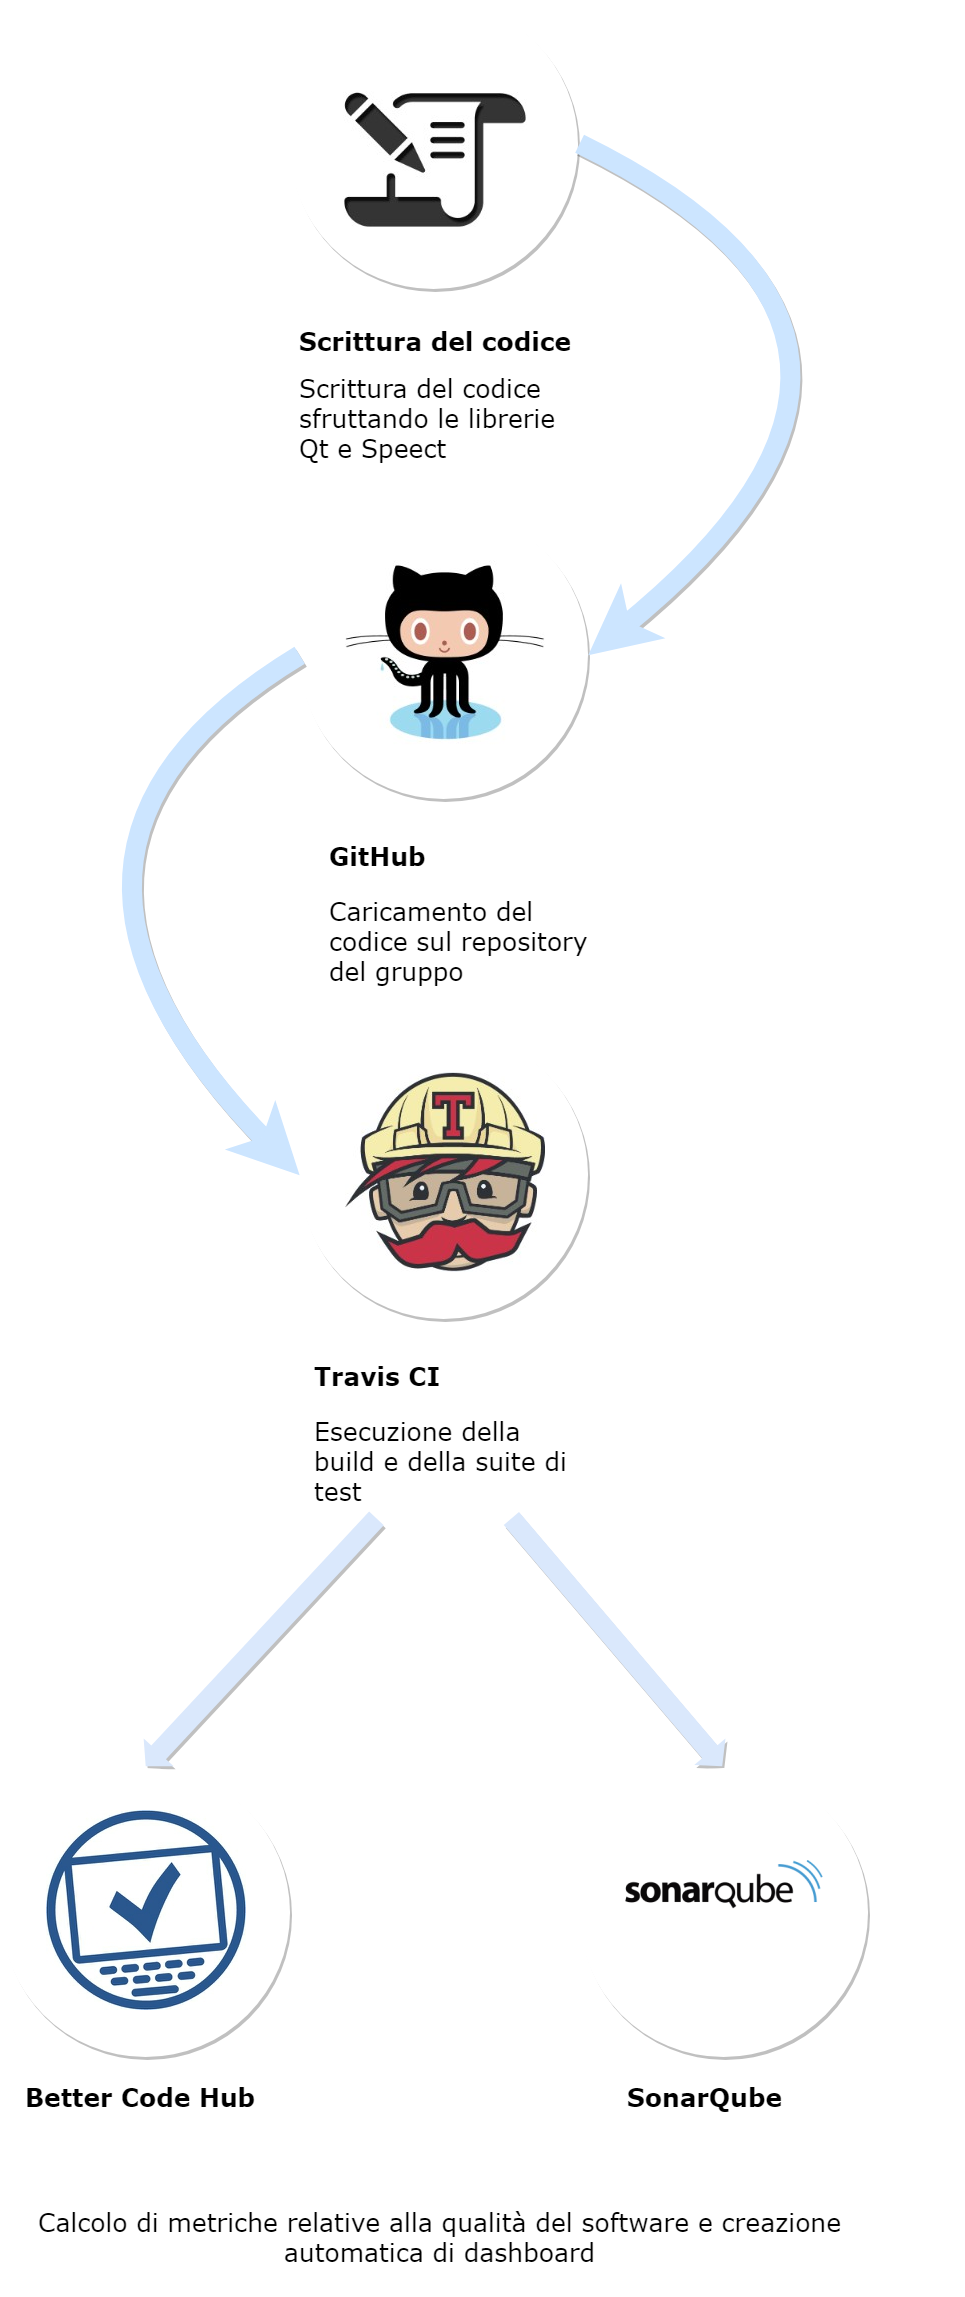
\includegraphics[scale=0.25]{CI}
	\centering
	\caption{Diagramma del flusso di integrazione continua}
\end{figure}

\end{document}
